\documentclass[12pt]{article}
\usepackage[top=1in, bottom=1in, left=.75in, right=.75in]{geometry}
\usepackage{amsmath, enumerate}
\usepackage{fancyhdr}
\usepackage{graphicx, xcolor, setspace}
\usepackage{txfonts}
\usepackage{multicol,coordsys,pgfplots}
\usepackage[scaled=0.86]{helvet}
\renewcommand{\emph}[1]{\textsf{\textbf{#1}}}
\usepackage{anyfontsize}
% \usepackage{times}
% \usepackage[lf]{MinionPro}
\usepackage{tikz,pgfplots}
\def\ra{\rightarrow}
\newcommand{\blank}[1]{\rule{#1}{0.75pt}}
\usetikzlibrary{calc,trees,positioning,arrows,fit,shapes,calc}
\pgfplotsset{width=9cm,compat=1.9}
\tikzset{
  jumpdot/.style={mark=*,solid},
  excl/.append style={jumpdot,fill=white},
  incl/.append style={jumpdot,fill=black},
}

\pgfplotsset{my style/.append style={axis x line=middle, axis y line=
middle, xlabel={$x$}, ylabel={$y$}}}

%axis equal

%yticklabels={,,} , xticklabels={,,}

% \setmainfont{Times}
% \def\sansfont{Lucida Grande Bold}
\parindent 0pt
\parskip 4pt
\pagestyle{fancy}
\fancyfoot[C]{\emph{\thepage}}
\fancyfoot[R]{v1} %%%%%% <-- Version Info
\fancyhead[L]{\ifnum \value{page} > 1\relax\emph{Math F251X: Midterm 1}\fi}
\fancyhead[R]{\ifnum \value{page} > 1\relax\emph{Fall 2025}\fi}
\headheight 15pt
\renewcommand{\headrulewidth}{0pt}
\renewcommand{\footrulewidth}{0pt}
\let\ds\displaystyle
\def\continued{{\emph {Continued....}}}
\def\continuing{{\emph {Problem \arabic{probcount} continued....}}\par\vskip 4pt}


\newcounter{probcount}
\newcounter{subprobcount}
\newcommand{\thesubproblem}{\emph{\alph{subprobcount}.}}
\def\problem#1{\setcounter{subprobcount}{0}%
\addtocounter{probcount}{1}{\emph{\arabic{probcount}.\hskip 1em(#1)}}\par}
\def\subproblem#1{\par\hangindent=1em\hangafter=0{%
\addtocounter{subprobcount}{1}\thesubproblem\emph{#1}\hskip 1em}}
\def\probskip{\vskip 10pt}
\def\medprobskip{\vskip 2in}
\def\subprobskip{\vskip 45pt}
\def\bigprobskip{\vskip 4in}


\newenvironment{subproblems}{%
\begin{enumerate}%
\setcounter{enumi}{\value{subprobcount}}%
\renewcommand{\theenumi}{\emph{\alph{enumi}}}}%
{\setcounter{subprobcount}{\value{enumi}}\end{enumerate}}


\newcommand{\be}{\begin{enumerate}}
\newcommand{\ee}{\end{enumerate}}


\begin{document}
{\emph{\fontsize{26}{28}\selectfont Fall 2025 \hfill
%{\fontsize{32}{36}\selectfont Calculus 1: Midterm 1}
\hfill Math F251X}}

\begin{center}
{\emph{%\fontsize{26}{28}\selectfont Spring 2024 
%%\hfill
{\fontsize{32}{36}\selectfont Calculus 1: Midterm 1}
%%\hfill Math F251X}
}}
\end{center}

%\vskip 2cm
\strut\vtop{\halign{\emph#\hskip 0.5em\hfil&#\hbox to 2in{\hrulefill}\cr
\emph{\fontsize{18}{22}\selectfont Name:}&\cr
%\noalign{\vskip 10pt}
%\emph{\fontsize{18}{22}\selectfont Student Id:}&\cr
%\noalign{\vskip 10pt}
%\emph{\fontsize{18}{22}\selectfont Calculator Model:}&\cr
}}
\hfill
\vtop{\halign{\emph{\fontsize{18}{22}\selectfont #}\hfil& \emph{\fontsize{18}{22}\selectfont\hskip 0.5ex $\square$ #}\hfil\cr
Section: & 9:15am (Kevin Meek)\cr
\noalign{\vskip 4pt}
         & 11:45am (James Gossell)\cr
\noalign{\vskip 4pt}
         & 11:45am (Margaret Short)\cr
\noalign{\vskip 4pt}
         & async (James Gossell)\cr}}
\vfill
{\fontsize{18}{22}\selectfont\emph{Rules:}}

\begin{itemize}
\item Partial credit will be awarded, but you must show your work.

\item You may have a single handwritten $3'' \times 5''$ notecard, both sides.

\item Calculators are {\bf not} allowed. 

\item Place a box around your \fbox{FINAL ANSWER} to each question where appropriate.

\item Turn off anything that might go beep during the exam.

\end{itemize}

%If you need extra space, you can use the back sides of the pages.
%Please make it obvious  when you have done so.



Good luck!
\vfill
\def\emptybox{\hbox to 2em{\vrule height 16pt depth 8pt width 0pt\hfil}}
\def\tline{\noalign{\hrule}}
\centerline{\vbox{\offinterlineskip
{
\bf\sf\fontsize{18pt}{22pt}\selectfont
\hrule
\halign{
\vrule#&\strut\quad\hfil#\hfil\quad&\vrule#&\quad\hfil#\hfil\quad
&\vrule#&\quad\hfil#\hfil\quad&\vrule#\cr
height 3pt&\omit&&\omit&&\omit&\cr
&Problem&&Possible&&Score&\cr\tline
height 3pt&\omit&&\omit&&\omit&\cr
&1&&16&&\emptybox&\cr\tline
&2&&9&&\emptybox&\cr\tline
&3&&9&&\emptybox&\cr\tline
&4&&10&&\emptybox&\cr\tline
&5&&8&&\emptybox&\cr\tline
&6&&6&&\emptybox&\cr\tline
&7&&12&&\emptybox&\cr\tline
&8&&12&&\emptybox&\cr\tline
&9&&18&&\emptybox&\cr\tline \tline
&Extra Credit&&(5)&&\emptybox&\cr\tline
&Total&&100&&\emptybox&\cr
}\hrule}}}

\newpage
%Graph problem
\problem{16 points} Consider the graph of the function $f(x)$ below.

%Begin picture
\begin{center}
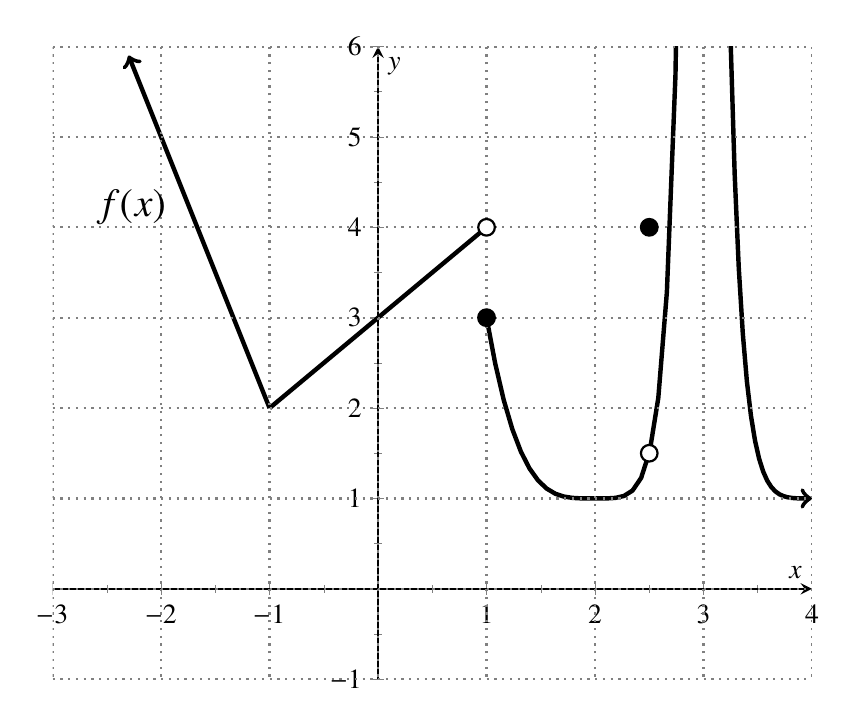
\begin{tikzpicture}
\begin{axis}[scale=1.3, thick, my style, xtick={-8,-7,...,8}, ytick={-8,-7,...,8},
xmin=-3, xmax=4, ymin=-1, ymax=6, minor y tick num=1,
        minor x tick num=1, mark size=3.0pt]
        \addplot[domain=-2.3:-1, smooth, ultra thick,<-] coordinates { (-2.3,5.9) (-1,2)};
        \addplot[domain=-1:1, smooth, ultra thick] coordinates {  (-1,2) (1,4)};
        \addplot[ultra thick,domain=1:2.9,->]{-4*(x - 2)^4/(x - 3)+1};
        \addplot[ultra thick,domain=3.1:4,->]{4*(x - 4)^4/(x - 3)+1};
\foreach \i in {-8,-7,-6,...,8}{
	\addplot[dotted, gray, domain=-8:8]{\i};
	\addplot[dotted, gray] coordinates {(\i,-8) (\i,8)};
	}
\addplot[mark=*,only marks] coordinates {(1,3)(2.5,4)};
 \addplot[mark=*,fill=white,only marks] coordinates {(1,4)(2.5,1.5)};
\end{axis}
\node at (1,6){{\Large{$f(x)$}}};
\end{tikzpicture}
\end{center}


Use the graph of $f(x)$ to answer each question below. If the limit is infinite, indicate
that with $\infty$ or $-\infty$. If the value does not exist or is undefined, write DNE.

\vspace{.2in}
\begin{tabular}{lll}
(a)  $\displaystyle{\lim_{x \rightarrow 1^-} f(x)} = $  \hspace{31mm} &  
(b) $\displaystyle{\lim_{x \rightarrow 1^+} f(x)} = $ \hspace{21mm} &  
(c) $\displaystyle{\lim_{x \rightarrow 1} f(x)} =  $
\\ \\ \\ \\
(d)  $\displaystyle{\lim_{h \rightarrow 0} \frac{ f(0+h)-f(0)}{h}} = $   &  
(e) $\displaystyle{\lim_{x \rightarrow 2} f'(x)} = $  &  
(f) $\displaystyle{\lim_{x \rightarrow -2} f'(x)} =  $
\\ \\ \\ \\
(g) $f(2.5) = $ & 
(h) $\displaystyle{\lim_{x \rightarrow 2.5} f(x)} = $  \hspace{31mm} &  
(i) $\displaystyle{\lim_{x \rightarrow 3} f(x)} = $  \hspace{31mm}
\end{tabular}

\vspace{.3in}
\,\, (j) Indicate {\bf{all}} $x$-values for which the function $f(x)$ is {\bf{not continuous}}:

\vspace{.3in}\hspace{.5in} \rule{3.8in}{.1mm}

\vspace{.1in}
\,\, (k) Indicate {\bf{all}} $x$-values for which the function $f(x)$ is {\bf{not differentiable}}:

\vspace{.4in}\hspace{.5in} \rule{3.8in}{.1mm}
\newpage

%Straight limit problems
\problem{9 points} Compute the following limits. Show your work. Use limit notation where necessary; you will be graded both on your computation and on your correct use of notation.

If the limit does not exist, write {\bf DNE} and a few words about why it does not exist. If the limit increases without bound, write $\infty$ or $-\infty$.
\begin{subproblems}
\item ${\displaystyle{\lim_{x \rightarrow 4^-} \, 
\frac{x^2-8x+15}{x^2-9x+20 }}}$ 
\vfill
\item ${\displaystyle{\lim_{x \rightarrow 2} \, 
\frac{ \frac{2}{x}-\frac{x}{2} }{x-2}}}$ 
\vfill
\item ${\displaystyle{  \lim_{\theta \rightarrow \pi/4 }  \frac{\sin^2 \theta}{\cos \theta}}}$ 
\vfill
\end{subproblems}


\newpage

% Continuity
\problem{9 points} Let 
\[f(x)=\begin{cases} \ds{\frac{5x^2+2x}{x}} & x < 0\\5 & x=0 \\ 5\sin(x)+2\cos(x) & x > 0 \end{cases}\]

\begin{subproblems}
	\item Evaluate $\ds{ \lim_{x \to 0^-} f(x)}$. Show supporting work.
	\vfill
	\vfill
	\item Evaluate $\ds{ \lim_{x \to 0^+} f(x)}$. Show supporting work.
	\vfill
	\vfill
	\item Evaluate $f(0)$. 
	\vfill
	\item Based on your answers to parts (a), (b) and (c), {\bf check the true statement(s) below}:
	\begin{enumerate}[$\Box$]
		\item $f$ is continuous at $x=0$.
		\item $f$ has a removable discontinuity at $x=0$.
		\item $f$ has a jump discontinuity at $x=0$.
		\item $f$ has an infinite discontinuity at $x=0$.
		\item None of the above.
	\end{enumerate}
	\vfill
\end{subproblems}

\newpage


\problem{10 points} Use the limit definition of the derivative (given below) to find the derivative of
$$
f(x) = \sqrt{x+3}
$$
Show all your work clearly using correct notation. {\bf No credit will
be awarded for a solution without adequate justification or that does
not use the definition below}.
$$
f'(x) = \lim_{h \rightarrow 0} \frac{f(x+h) - f(x)}{h}
$$
\vfill

\vfill
\vfill
\vfill
\vfill
\vfill

\newpage

\problem{8 points} The function $y=H(x)$ is graphed below. Sketch the graph
of $H'(x)$ on the blank set of axes provided.

\begin{multicols}{2}
\begin{center}
		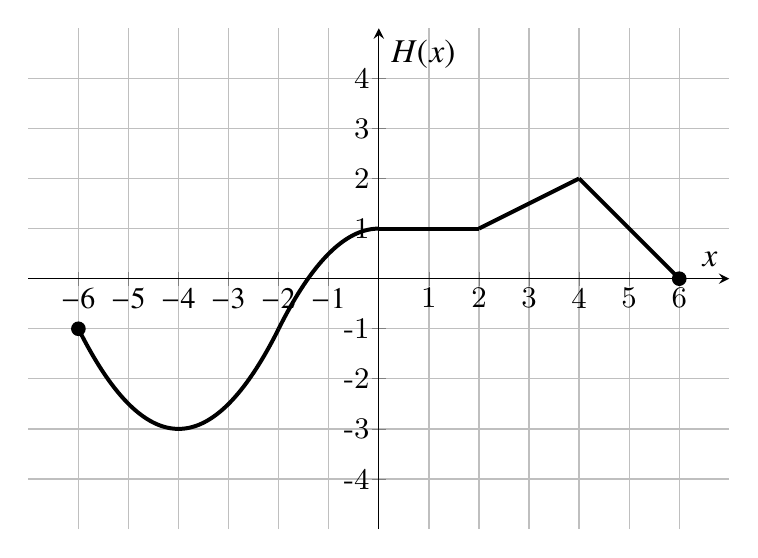
\begin{tikzpicture}[scale=1.2]
		\begin{axis}[
		axis lines=middle,
		unit vector ratio=1 1 1,
		grid=major,
		xmin=-7,
		xmax=7,
		ymin=-5,
		ymax=5,
		xlabel=$x$,
		ylabel=$H(x)$,
		xtick={-6,-5,...,5,6},
		xticklabels={ $-6$,$-5$,$-4$,$-3$,$-2$,$-1$,0,1,2,3,4,5, 6},
		ytick={-4,-3,...,3,4},
		yticklabels={-4,-3,-2,-1,0,1,2 ,3,4},
		yticklabel style = {xshift=0.1cm},
		xticklabel style = {yshift=0.1cm},
		tick label style={font=\small},
		legend style={
			at={(rel axis cs:0,1)},
			anchor=north west,draw=none,inner sep=0pt,fill=gray!10}
		]
		\addplot[-,domain=(-6:-2), black, very thick, samples=100] {(1/2)*(x+4)^2-3};
		\addplot[-,domain=(-2:0), black, very thick, samples=100] {-(1/2)*(x-0)^2+1};
		\addplot[-,domain=(0:2), black, very thick, samples=100] {1};
		\addplot[-,domain=(2:4), black, very thick, samples=100] {x/2};
		\addplot[-,domain=(4:6), black, very thick, samples=100] {-x+6};
		\addplot[incl] coordinates {(-6,-1)};
		\addplot[incl] coordinates {(6,0)};
		\end{axis}
		\end{tikzpicture}
\end{center}
%\vspace{2cm}

\begin{center}
		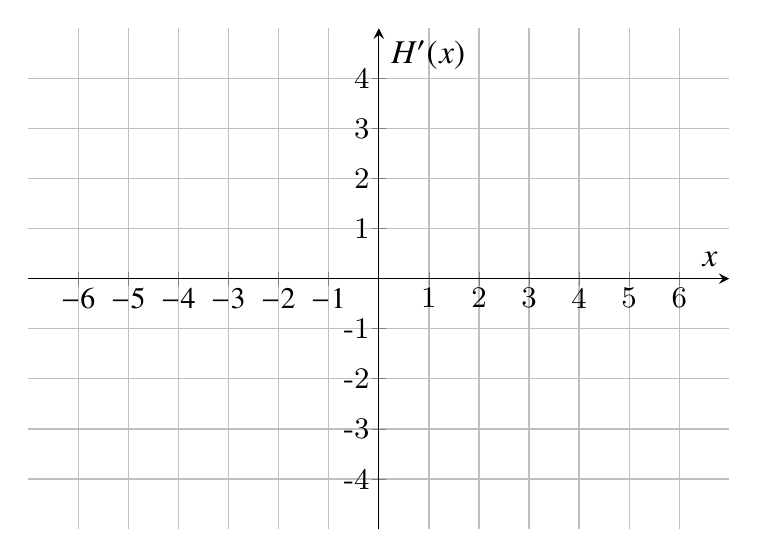
\begin{tikzpicture}[scale=1.2]
		\begin{axis}[
		axis lines=middle,
		unit vector ratio=1 1 1,
		grid=major,
		xmin=-7,
		xmax=7,
		ymin=-5,
		ymax=5,
		xlabel=$x$,
		ylabel=$H'(x)$,
		xtick={-6,-5,...,5,6},
		xticklabels={ $-6$,$-5$,$-4$,$-3$,$-2$,$-1$,0,1,2,3,4,5, 6},
		ytick={-4,-3,...,3,4},
		yticklabels={-4,-3,-2,-1,0,1,2 ,3,4},
		yticklabel style = {xshift=0.1cm},
		xticklabel style = {yshift=0.1cm},
		tick label style={font=\small},
		legend style={
			at={(rel axis cs:0,1)},
			anchor=north west,draw=none,inner sep=0pt,fill=gray!10}
		]
		\end{axis}
		\end{tikzpicture}
\end{center}
\end{multicols}

\vspace{0.2cm}

%Derivative Application
\problem{6 points} $S(t)$ is a function that describes the number of survivors in UAF's annual Humans vs. Zombies game, $t$ days after the start of the game.
	\begin{subproblems}
	\item Interpret the meaning of \fbox{$S(2)=235$} in the context of the problem. Write a sentence or two including appropriate units. 
	
	\vfill
	
	\item Interpret the meaning of \fbox{$S'(2)=-53$} in the context of the problem. Write a sentence or two including appropriate units. 
	
	\vfill
	
	\item Using parts (a) and (b), \emph{estimate} $S(3)$ including units. Write a sentence explaining how you arrived at your estimation.
	
	\vfill
\end{subproblems}

  % \problem{1} What can you say about $f'(3)$ if $\ds f(x) = \frac{e^{\sin(4x^5-3x^2-1)}\ln(\sqrt{x+32})}{x-3}$? (maybe bonus?)

  % \problem{1} BONUS: Note that $\ds \tan\left(\frac{\pi}{3}\right) =
  % \sqrt{3}$ and $\ds \tan\left(\frac{5\pi}{3}\right) = -\sqrt{3}$. Does
  % the Intermediate Value Theorem guarantee that $f(x) = \tan(x)$ has a
  % zero on the interval $\ds
  % \left[\frac{\pi}{3},\frac{5\pi}{3}\right]$? Why or why not?


\newpage

%Straight derivative problems
\problem{12 points}  Compute the {\bf derivative} of each of the following functions using any method you like. \emph{You do not need to simplify your answers.}
\begin{subproblems}
\item $\ds g(x) = x^{3.4} - \frac{2}{3x^2} + \sqrt{x} - \sin\left(\frac{\pi}{2}\right)$
  \vfill

\item $\ds f(x) = \cos(x) \left( 4x^5 - 3x^2 \right)$
  \vfill

\item $\ds h(\theta) = \frac{\sin(\theta)}{\theta}$
  \vfill

\item $\ds s(x) = x^2(\sin x)(\cos x)$
  \vfill
\end{subproblems}

\newpage


\newpage


%%%%%  tangent lines
\problem{12 points} The function $g(x) = x^2(x-1)+4$ is graphed below.

\begin{center}
\begin{tikzpicture}[yscale=0.5,xscale=1.8]
  \draw[->] (-2.5, 0) -- (2.5, 0) node[right] {$x$};
  \draw[->] (0, -7) -- (0, 10) node[above] {$g(x)$};
  \draw[<->, domain=-1.9:1.9, smooth, variable=\x, ultra thick] plot ({\x}, {\x*\x*(\x-1)+5});
  \foreach \i in {-2,-1,1,2}{
  	\draw (\i,-.5)--(\i,0.5);
	\node at (\i,-1.3){\i};
	}
%\draw (-.1,25)--(0.1,25);
%\node at (-0.5,25){25};
\end{tikzpicture}
\end{center}

\begin{subproblems}
\item Sketch and label the graph of the {\bf tangent line} to the
  graph of $g(x)$ when $x=-1$.
  \vspace{1cm}
  
\item Write an equation for the tangent line to $g(x)$ when $x=-1$.
  \vfill
  
\item Find all the $x$-values at which the graph of $g(x)$ has a
  horizontal tangent line or explain why none exist. Justify your
  answer and show your work.
  \vfill
\end{subproblems}


\newpage
%%%%%%%%%% velocity and stuff




\problem{18 points} An NFL quarterback throws a football straight up from the surface of the moon. While the football is in the air, its height in meters after $t$ seconds is $h(t)=t(28-0.8t)$
	\begin{subproblems}
	\item Find functions describing the \emph{velocity} and \emph{acceleration} of the football.
	
	\vfill
	
	\item What was the \emph{initial velocity} of the football? Include correct units in your answer.
	
	\vfill
	
	\item After $10$ seconds, is the football speeding up or slowing down? Show your work and justify your answer.
	
	\vfill

	\item When does the football reach its highest point? Include correct units in your answer.
	
	\vfill
	
	\item When does the fooball hit the ground? Include correct units in your answer.
	
	\vfill

	\item What is the \emph{acceleration due to gravity} on the surface of the moon? Include correct units in your answer.
	
	\vfill 
	\end{subproblems}

\newpage


%\fbox{Extra Credit} 
\problem{Extra Credit: 5 points}

\vspace{.3in}



Is it always true that $\displaystyle\frac{d}{dx} \left[ \frac{f(x)}{g(x)} \right] = \frac{f'(x)}{g'(x)}\,$?\\

If so, explain why. If not, provide an example where $\displaystyle\frac{d}{dx} \left[ \frac{f(x)}{g(x)} \right] \ne \frac{f'(x)}{g'(x)}$.\\



\end{document}

%%%%ENDDOCUMENT


